
La température cinétique d'un système autogravitant est la valeur moyenne dans l'espace des positions du carré de la
vitesse d'une particule test. Comme $\vec p = m\vec v $, si $f(\vec r, \vec p, t)$ est la fonction de distribution de ce
système et $\rho(\vec r , t)= \int f(\vec r, \vec p, t) d\vec p$ sa densité, alors sa température cinétique $T(\vec r ,
t)$ est définie par la relation
\begin{align}
	T(\vec r , t)=\dfrac{\int v^2 f(\vec r, \vec p, t) d\vec p}{\int f(\vec r, \vec p, t) d\vec p}=\dfrac{1}{m\rho(\vec r, t)} \int p^2 f(\vec r, \vec p, t) d\vec p
\end{align}
Un rapide calcul montre que dans la cas de la sphère isotherme~\refeq{sph-iso}, la température $T(\vec r ,
t)=(k_B\beta)^{-1}$ est constante en chaque point, d'où le nom de ce système. Nous avons vu que la sphère de King peut s'apparenter à
une sphère isotherme tronquée en énergie, étudions l'influence de cette troncature sur la température.
 
\subsection{Calcul de la température en chaque point}

Dans le cas de la fonction de distribution de King, nous avons:
\begin{align}
	\int_0^{p_l} p^2 f_K\(E\) d\vec{p} 
	=
	4\pi \dfrac{\rho_0}{\(2\pi m\sigma^2\)^{3/2}} \int_0^{p_l}\( e^{\frac{E_l-E}{\sigma^2}} - 1\)  p^4 \ddp 
\end{align}
% Puisque l'énergie moyenne par particule $E = \dfrac{p^2}{2m} + m\psi$ ne dépend que des modules $r$ de $\vec r$ et $p$
% de $\vec p$, la température ne dépend spatialement que de $r$. Nous avions vu que
avec $p_l = \sqrt{2m\(E_l - m\psi(r)\)} =
\sqrt{2m\phi(r)}$. Une intégration par parties et quelques lignes de calcul donnent alors directement:
\begin{align}
	\begin{split}
		\int_0^{p_l} p^2 f_K\(E\) d\vec{p} =
		\frac{4\pi\rho_0}{m^2\(2\pi m\sigma^2\)^{3/2}}
				\(
					\dfrac{3}{2} \(m\sigma^2\)^2\sqrt{2m\pi\sigma^2}
					\left[
						e^{\frac{\phi}{\sigma^2}}\erf\(\sqrt{\dfrac{\phi(r)}{\sigma^2}}\)
						\right. \right.\\
						\left. \left.
						- \sqrt{\dfrac{4\phi(r)}{ \pi\sigma^2}}
						\(1 + \dfrac{2\phi(r)}{3\sigma^2}\)
					\right]
					- \dfrac{\(2m\phi(r)\)^{5/2}}{5}
				\) 
	\end{split}
% \int_0^{p_l} p^2 f_K\(E\) d\vec{p} =
% \frac{4\pi\rho_0}{m^2\(2\pi m\sigma^2\)^{3/2}}
		% \(
			% \dfrac{3}{2} \(m\sigma^2\)^2\sqrt{2m\pi\sigma^2}
			    % \left[
				% e^{\frac{\phi}{\sigma^2}}\erf\(\sqrt{\dfrac{\phi(r)}{\sigma^2}}\)
			% \right. \right. \notag \\
	    % \left.\vphantom{\(\sqrt{\dfrac{\phi(r)}{\sigma^2}}\) }\left.\vphantom{\(\sqrt{\dfrac{\phi(r)}{\sigma^2}}\)}
				% - \sqrt{\dfrac{4\phi(r)}{ \pi\sigma^2}}
				% \(1 + \dfrac{2\phi(r)}{3\sigma^2}\)
			% \right]
			% - \dfrac{\(2m\phi(r)\)^{5/2}}{5}
		% \) 
\end{align}

Nous en déduisons la température cinétique de la sphère de King en divisant par le produit $m\rho$; après quelques
simplifications et en utilisant la fonction $\gamma(r)=\phi(r)/\sigma^2$,  il vient:
\begin{align}
	T_K (r) 
	= \dfrac{3\sigma^2}{m}	
		\(
			1
		- 
		\dfrac{8}{15 \sqrt{\pi}}
		\(\dfrac{\rho(r)}{\rho_0}\)^{-1}\(\gamma(r)\)^{5/2}
		\)
\end{align}
Cette expression n'est pas très explicite mais son calcul numérique ne présente pas de difficulté dès lors que l'on a
déterminé, numériquement aussi, la fonction $\phi(r)$. Il s'avère intéressant de tracer la fonction:
\begin{align*}
	\zeta(r)=\(\dfrac{\rho(r)}{\rho_0}\)^{-1}\(\gamma(r)\)^{5/2}
\end{align*}
et de la comparer avec la valeur $1$. C'est l'objet de
la figure~\ref{Fig::King::ZetaFunc}. Outre le facteur $\dfrac{8}{15 \sqrt{\pi}}\approx 0.3$, nous remarquons que 
la température $T(r)$ est quasiment constante sur dans les régions ou la densité est importante
($\frac{\rho(r)}{\rho_0}>10^{-5}$ pour $W_0=15$).
% Cette expression n'est pas très explicite mais son calcul numérique ne présente pas de difficulté dès lors que l'on a
% déterminé, numériquement aussi, la fonction $\phi(r)$. Il s'avère intéressant de tracer la fonction
% $$\zeta(r)=\(\dfrac{\rho(r)}{\rho_0}\)^{-1}\(\gamma(r)\)^{5/2}$$ et de la comparer avec la valeur $1$. C'est l'objet de
% la figure \ref{Fig::King::ZetaFunc}. Outre le facteur $\dfrac{8}{15 \sqrt{\pi}}\approx 0.3$, nous remarquons que pour des valeurs
% de $W_0\leq15$, la température $T(r)$ est quasiment constante sur dans les régions ou la densité est importante
% ($\frac{\rho(r)}{\rho_0}>10^{-5}$ pour $W_0=15$ et bien mieux pour les valeurs de $W_0$ plus faibles).

% \begin{figure}[hbt]
	% \centering 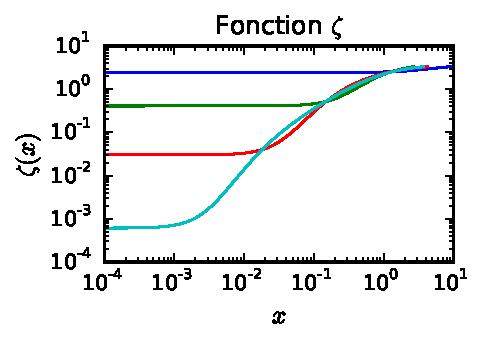
\includegraphics{graphe/king_t.pdf}
	% \caption{Température d'un modèle de King: la fonction $\zeta(r)$. Le code couleur est le même que pour la figure~\ref{King_Modele-test}\label{Fig::King::ZetaFunc}}
% \end{figure}
\begin{figure}[hbt]
	\centering 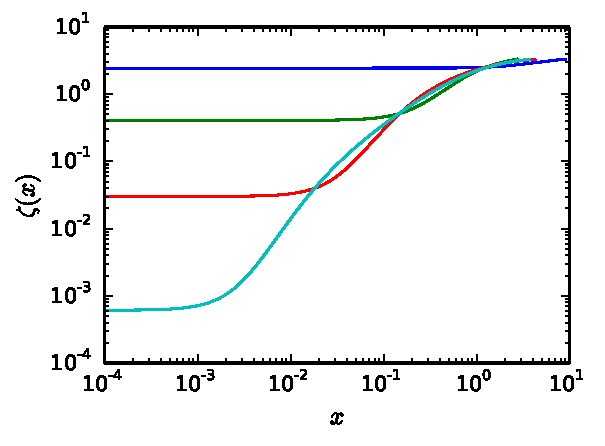
\includegraphics{graphe/zeta_func.pdf}
	\caption{Température d'un modèle de King: la fonction $\zeta(r)$. Le code couleur est le même que pour la figure~\ref{King_Modele-test}\label{Fig::King::ZetaFunc}}
\end{figure}

\begin{figure}[hbt]
	\begin{minipage}[b]{0.48\linewidth}
		\centering 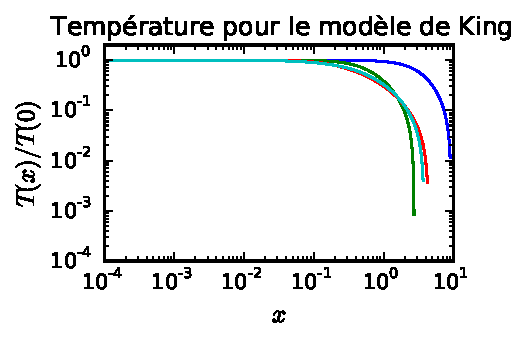
\includegraphics{graphe/king_n_t_temp.pdf}
	\end{minipage}\hfill
	\begin{minipage}[b]{0.48\linewidth}
		\centering 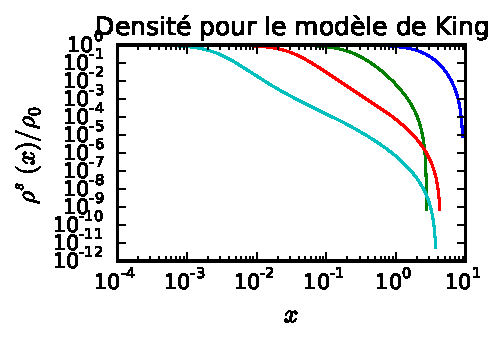
\includegraphics{graphe/king_n.pdf}
	\end{minipage}
	\caption{Température et densité d'un modèle de King: les fonctions $\frac{T(x)}{T(0)}$ et
		$\frac{\rho(x)}{\rho(0)}$. Le code couleur est le même que pour la figure~\ref{King_Modele-test}}
	\label{kingisotherme}
\end{figure}

À partir de maintenant, nous assimilerons un modèle de King à une sphère isotherme.

% \begin{figure}[H]
	% \begin{minipage}[b]{0.40\linewidth}
		% \centering \includegraphics[scale=0.40]{theorie/graphe/Courbes_temperature_KING.pdf}
	% \end{minipage}\hfill
	% \begin{minipage}[b]{0.48\linewidth}
		% \centering \includegraphics[scale=0.40]{theorie/graphe/Courbes_densite_KING.pdf}
	% \end{minipage}
	% \caption{Température d'un modèle de King : les fonctions $\zeta(r)$ et $\rho(r)$.}
	% \label{kingisotherme}
% \end{figure}


\subsection{Température moyenne d'un modèle de \King}
\label{Calc::Temp}

Hormis le cas particulier  de la sphère isotherme, la température cinétique est une fonction de la position\footnote{Il s'agit même d'une fonction du
temps si le système est hors de l'équilibre. Dans ce cas la notion de température perd un peu de son sens.}. Nous pouvons tout de même définir une
température moyenne en intégrant la température cinétique dans l'espace des positions. Nous prendrons par exemple et par définition:
\begin{align}
T_{\mathrm{moy}} = \dfrac{\displaystyle{\int}\frac{p^2}{m^2}f(\vec r, \vec p, t) d\vec p d\vec r}
                                        {\displaystyle{\int} f(\vec r, \vec p, t) d\vec p d\vec r}
\end{align}
Il est clair que pour la sphère isotherme $T_{\mathrm{moy}}=T(r)=T$; pour la sphère de King un calcul final montre que:
\begin{align}
	    T_{K,\mathrm{moy}}
	    = \frac{3\sigma^2}{m} - \frac{32\pi^2\rho_0}{5 M m\(\pi \sigma^2\)^{3/2}}\displaystyle{\int}_0^R r^2 \(\phi(r)\)^{5/2}
			dr
\end{align}
Cette relation montre que la température moyenne d'un modèle de King est toujours inférieure à celle des modèles de sphère isotherme vus précédemment.

\begin{figure}[h!]
	\centering 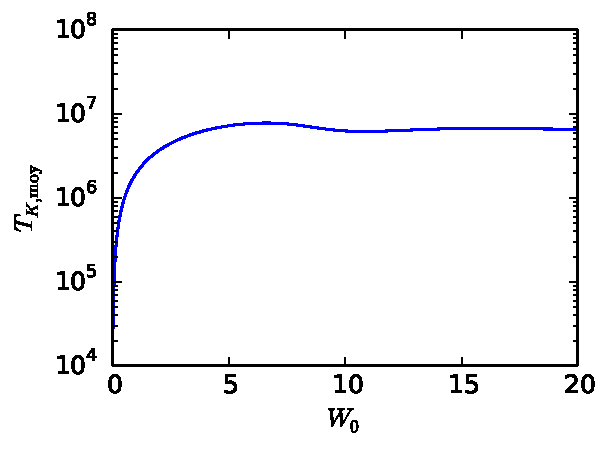
\includegraphics{graphe/king_temperature_moy_v3.pdf}
	% \centering 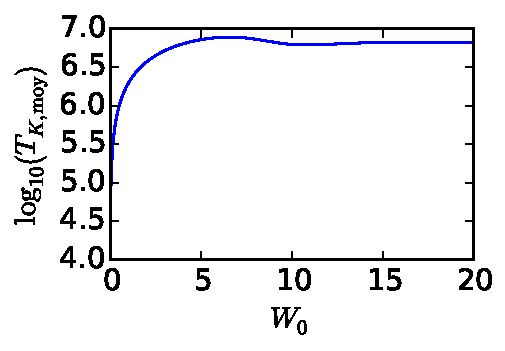
\includegraphics{graphe/king_temperature_moy_v2.pdf}
	% \centering \includegraphics[width=1.00\textwidth]{theorie/graphe/Temperature_centre-moyenne.pdf}
	\caption{Température moyenne en fonction de $W_0$\label{courbe::Moy}}
\end{figure}
La courbe~\ref{courbe::Moy} présente la variation de la température moyenne. Il est intéressant de noter que pour $W_0$ dans
l'intervalle $[5; 20]$ la température moyenne ne varie plus, nous confirmant ce que l'on pouvait voir sur la
figure~\ref{kingisotherme}: passé une valeur de $W_0$, tous les King semblent avoir la même température.

